\documentclass[tikz,border=5pt]{standalone}
\usepackage[T1]{fontenc}
\usepackage{lmodern,amsmath,amssymb}
\usetikzlibrary{arrows.meta,calc,positioning,fit,backgrounds,shapes.geometric,matrix,decorations.pathreplacing,patterns}
\definecolor{ink}{gray}{0.08}
\definecolor{wash}{gray}{0.965}
\definecolor{soft}{gray}{0.45}
\tikzset{box/.style={draw=ink,line width=.65pt,fill=white,align=center,inner sep=4pt,outer sep=0pt,font=\small},flow/.style={draw=ink,line width=.65pt,-{Latex[length=1.8mm,width=1.3mm]},rounded corners=2pt},annotation/.style={font=\scriptsize,text=soft,align=center},groupbox/.style={draw=soft,dashed,line width=.45pt,fill=wash}}
\begin{document}
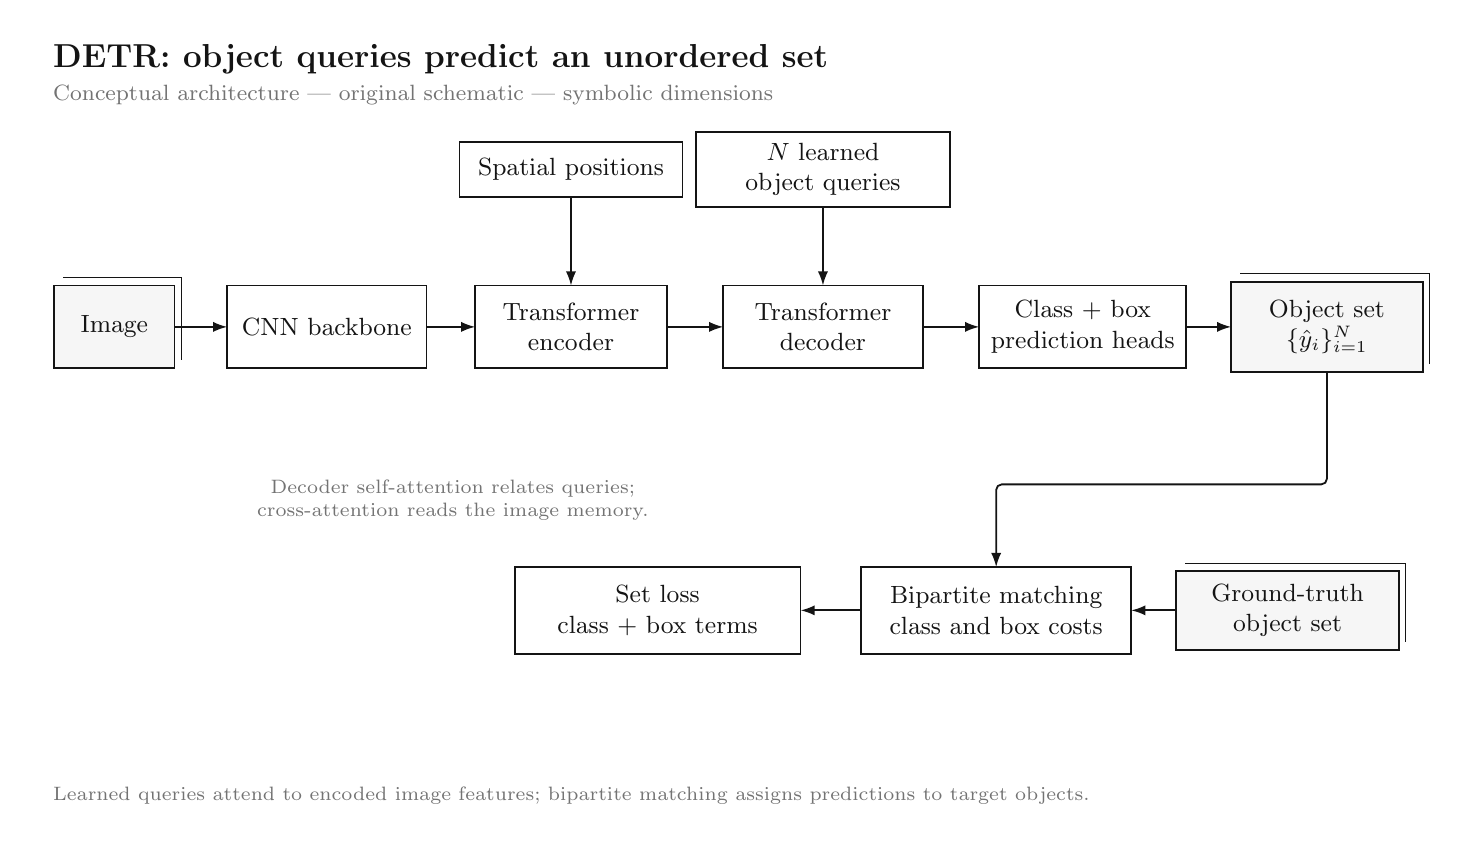
\begin{tikzpicture}[x=1cm,y=-1cm,font=\rmfamily,text=ink]

\path[use as bounding box] (0,0) rectangle (18,10);
\node[anchor=west,font=\large\bfseries] at (.2,.4) {DETR: object queries predict an unordered set};
\node[anchor=west,font=\footnotesize,text=soft] at (.2,.85) {Conceptual architecture | original schematic | symbolic dimensions};
\begin{pgfonlayer}{background}
\end{pgfonlayer}
\node[box,fill=wash,minimum width=1.5cm,minimum height=1.05cm,text width=1.25cm] (x) at (1.1,3.8) {Image};
\draw[ink,line width=.4pt] (0.45000000000000007,3.175) -- (1.9500000000000002,3.175) -- (1.9500000000000002,4.2250000000000005);
\node[box,minimum width=2.5cm,minimum height=1.05cm,text width=2.25cm] (cnn) at (3.8,3.8) {CNN backbone};
\node[box,minimum width=2.4cm,minimum height=1.05cm,text width=2.15cm] (enc) at (6.9,3.8) {Transformer\\encoder};
\node[box,minimum width=2.5cm,minimum height=1.05cm,text width=2.25cm] (dec) at (10.1,3.8) {Transformer\\decoder};
\node[box,minimum width=2.6cm,minimum height=1.05cm,text width=2.35cm] (head) at (13.4,3.8) {Class + box\\prediction heads};
\node[box,fill=wash,minimum width=2.4cm,minimum height=1.15cm,text width=2.15cm] (set) at (16.5,3.8) {Object set\\$\{\hat y_i\}_{i=1}^{N}$};
\draw[ink,line width=.4pt] (15.4,3.1249999999999996) -- (17.8,3.1249999999999996) -- (17.8,4.275);
\node[box,minimum width=2.8cm,minimum height=0.7cm,text width=2.55cm] (pos) at (6.9,1.8) {Spatial positions};
\node[box,minimum width=3.2cm,minimum height=0.7cm,text width=2.95cm] (queries) at (10.1,1.8) {$N$ learned\\object queries};
\node[box,fill=wash,minimum width=2.8cm,minimum height=1.0cm,text width=2.55cm] (gt) at (16.0,7.4) {Ground-truth\\object set};
\draw[ink,line width=.4pt] (14.7,6.800000000000001) -- (17.5,6.800000000000001) -- (17.5,7.800000000000001);
\node[box,minimum width=3.4cm,minimum height=1.1cm,text width=3.15cm] (match) at (12.3,7.4) {Bipartite matching\\class and box costs};
\node[box,minimum width=3.6cm,minimum height=1.1cm,text width=3.35cm] (loss) at (8.0,7.4) {Set loss\\class + box terms};
\begin{pgfonlayer}{background}
\draw[flow] (x.east) -- (cnn.west);
\draw[flow] (cnn.east) -- (enc.west);
\draw[flow] (enc.east) -- (dec.west);
\draw[flow] (dec.east) -- (head.west);
\draw[flow] (head.east) -- (set.west);
\draw[flow] (pos.south) -- (enc.north);
\draw[flow] (queries.south) -- (dec.north);
\draw[flow] (set.south) -- (16.5,5.8) -- (12.3,5.8) -- (match.north);
\draw[flow] (gt.west) -- (match.east);
\draw[flow] (match.west) -- (loss.east);
\end{pgfonlayer}
\node[annotation,text width=8.0cm] at (5.4,6.0) {Decoder self-attention relates queries; cross-attention reads the image memory.};
\node[anchor=west,align=left,font=\scriptsize,text=soft,text width=17.6cm] at (.2,9.75) {Learned queries attend to encoded image features; bipartite matching assigns predictions to target objects.};
\end{tikzpicture}
\end{document}
